\documentclass{article}
\usepackage{graphicx} % Required for inserting images

\title{Exercises}
\author{Yakup Kaan Baycan}
\date{July 2023}

\begin{document}

\maketitle

\section{2.4 Statistical Learning Exercises}
\subsection{Conceptual}
\subsubsection{} For each of parts (a) through (d), indicate whether we would generally expect the performance of a flexible statistical learning method to be better or worse than an inflexible method. Justify your answer.\\

\textbf{(a) The sample size n is extremely large, and the number of predictors p is small.} \\

Since n is large, and p is small we tend to use a \textbf{flexible model}. Although a flexible model will not perfectly fit to data it is better compared to inflexible models. Hence, an inflexible model will require more parameters to fit, and as the model gets more complex and flexible we may face \textbf{over-fitting problem} \\

\textbf{(b) The number of predictors p is extremely large, and the number
of observations n is small.}\\

In this case, we may go with an \textbf{inflexible model} since we do not have enough data to train. An inflexible model behaves better with a small n and reduces the risk of over-fitting.\\

\textbf{(c) The relationship between the predictors and response is highly
non-linear.}\\

If we are aware that the response variable is non-linear, then using a \textbf{flexible model} will be more accurate since it performs well when there is non-linearity. Hence, an inflexible model will have a higher bias which will result in a worse score.\\

\textbf{(d) The variance of the error terms, i.e. $\sigma^2$ = $Var(\epsilon)$, is extremely high.}\\

In such case, we may use the formula MSE = $Bias(\hat{y})^2 + Var(\hat{y})$. If the variance of the error terms is extremely high, the flexible model may overfit easily and fail on the test set. So we should go with an \textbf{inflexible model} which may seem less accurate in the training set but will perform better than a flexible one on new data.\\

\subsubsection{} Explain whether each scenario is a classification or regression problem, and indicate whether we are most interested in inference or prediction. Finally, provide n and p.\\

\textbf{(a) We collect a set of data on the top 500 firms in the US. For each firm we record profit, number of employees, industry and the CEO salary. We are interested in understanding which factors affect CEO salary.}\\

Here we are interested in the factors rather than how to estimate a new CEO salary. Hence, we are most interested in inference and the correlation between the variables and the response. n = 500 p = 3 and it is a regression problem. \\

\textbf{(b) We are considering launching a new product and wish to know whether it will be a success or a failure. We collect data on 20
similar products that were previously launched. For each product, we have recorded whether it was a success or failure, the price charged for the product, the marketing budget, the competition price, and ten other variables.}\\

This problem is a binary classification problem in which the possible outcome matters more than the effects of predictors. Hence, the prediction matters most. n = 20, p = 13 \\

\textbf{(c)We are interested in predicting the change in the USD/Euro exchange rate in relation to the weekly changes in the world stock markets. Hence we collect weekly data for all of 2012. For each week we record the change in the USD/Euro, the change in the US market, the change in the British market, and the change in the German market.} \\

As mentioned in the first sentence, aim is to predict the change in USD/Euro exchange rate, and there are two possibilities. First, it may be a binary classification problem with outcomes up and down or it may be a regression problem which we decide on whether it went up or down.
n = 52, p = 3.

\subsubsection{} We now revisit the bias-variance decomposition.

\textbf{(a) Provide a sketch of typical (squared) bias, variance, training error,
test error, and Bayes (or irreducible) error curves, on a single plot, as we go from less flexible statistical learning methods towards more flexible approaches. The x-axis should represent the amount of flexibility in the method, and the y-axis should represent the values for each curve. There should be five curves. Make sure to label each one.}

\subsubsection{} You will now think of some real-life applications for statistical learning. \\

\textbf{(a) Describe three real-life applications in which classification might
be useful. Describe the response, as well as the predictors. Is the goal of each application inference or prediction? Explain your answer. }\\

Cancer type detection, financial market behavior, customer churn analysis. For the first one, the main goal is to predict whether a cell is benign or malign which is the response, and other factors like age, sex etc as predictors.
For the second one, the main goal is again to predict the behavior. Although, we may be interested in how other factors such as interest rate, the company's ROI, and other financials affect the response.
Lastly, customer churn analysis helps companies to detect which customers are most likely to leave and take action towards. Again we are more interested in the prediction rather than inference here.\\

\textbf{(b) Describe three real-life applications in which regression might
be useful. Describe the response, as well as the predictors. Is the  goal of each application inference or prediction? Explain your answer.}\\

Price of anything(house, car, materials), profit, sales. Price analysis seems to be the most wide use area of regression since it helps to predict a price for both selling and buying a property. 
Secondly, the profit of a company is another use case in which inference is more important than prediction. With the inference between variables and the response, a company may choose to change its focus on specific areas.
Lastly, sales is another use case for companies to both see which tool increases sales and predict the next quarter's sales. So both, inference and prediction matter equally.\\

\textbf{(c) Describe three real-life applications in which cluster analysis
might be useful.}\\

Customer segmentation, disease prediction(more than 2), and image prediction.
Customer segmentation helps companies to come up with special campaigns and promotions for different types of customers. For example a flight promotion for a businessman, and a book campaign for a student. 
For disease prediction, by putting the input of old patients and their data, we may just use a model to predict the best-fitting possible outcomes and fasten the process of diagnosing.
Lastly, we may predict the number or the letter in an image by cluster analysis.\\

\subsubsection{} \textbf{What are the advantages and disadvantages of a very flexible (versus
a less flexible) approach for regression or classification? Under what circumstances might a more flexible approach be preferred to a less flexible approach? When might a less flexible approach be preferred?} \\

Flexible methods have many advantages. Firstly, a flexible method with a large dataset in which the response variable is mostly non-linear may perform much better than an inflexible method. The large dataset also deters overfitting problems. Also, flexible methods take more parameters into account. As a result, we end up analyzing more predictors.

\subsubsection{}\textbf{Describe the differences between a parametric and a non-parametric statistical learning approach. What are the advantages of a parametric approach to regression or classification (as opposed to a nonparametric approach)? What are its disadvantages?} \\

Parametric methods are more easy to interpret although it is more biased than non-parametric methods. Also, non-parametric methods require more predictors than parametric methods and become a black box that is hard to interpret. Another difference between them is guessing the form of true f. Parametric methods assume the form of the true f, such as linear. On the other hand, non-parametric methods avoid this by not making major assumptions about the form of true f.


\subsubsection{} The table below provides a training data set containing six observations,
three predictors, and one qualitative response variable
\begin{table}[htbp]
  \centering
  \caption{Observations} 
  \label{tab:example}
  \begin{tabular}{|c|c|c|c|c|}
    \hline
    \textbf{Obs.} & \textbf{$X_1$} & \textbf{$X_2$} &\textbf{$X_3
    $} & \textbf{Y} \\
    \hline
    1 & 0 & 3 & 0 & Red \\
    \hline
    2 & 2 & 0 & 0 & Red \\
    \hline
    3 & 0 & 1 & 3 & Red\\
    \hline
    4 & 0 & 1 & 2 & Green\\
    \hline
    5 & -1 & 0 & 1 & Green \\
    \hline
    6 & 1 & 1 & 1 & Red\\
    \hline
  \end{tabular}
\end{table} \\
Suppose we wish to use this data set to make a prediction for Y when X1 = X2 = X3 = 0 using K-nearest neighbors.\\

\textbf{(a) Compute the Euclidean distance between each observation and the test point, $X_1 = X_2 = X_3 = 0.$ }
Let's calculate respectively: \\
$D_1 = \sqrt{((0-0)^2+(3-0)^2+(0-0)^2)} = 3$\\
$D_2 = \sqrt{((2-0)^2+(0-0)^2+(0-0)^2)} = 2$\\
$D_3 = \sqrt{((0-0)^2+(1-0)^2+(3-0)^2)} = \sqrt{10}$\\
$D_4 = \sqrt{((0-0)^2+(1-0)^2+(2-0)^2)} = \sqrt{5}$\\
$D_5 = \sqrt{((-1-0)^2+(0-0)^2+(1-0)^2)} = \sqrt{2}$\\
$D_6 = \sqrt{((1-0)^2+(1-0)^2+(1-0)^2)} = \sqrt{3}$\\

\textbf{(b) What is our prediction with K = 1? Why? }\\

If we take K=1, that means we choose class as the closest training data which is $min(D_1,D_2,D_3,D_4,D_5,D_6)$. Hence the closest neighbor is the 5th observation. So the prediction is \textit{Green}. \\ 

\textbf{(c) What is our prediction with K = 3? Why? }\\

If we change K to 3. Then we first find the 3 closest neighbors which are: $D_5, D_6, D_2$. Their responses are respectively, Green, Red, Red. So we predict as \textit{Red}. \\

\textbf{(d) If the Bayes decision boundary in this problem is highly nonlinear, then would we expect the best value for K to be large or
small? Why?} \\

If the problem is highly non-linear then we must use a more flexible method to get the best result. Hence, usage of small K will be the right choice, since as K goes to n there occurs a linear bound which is not good for non-linear problems.

\subsection{Applied}
\subsubsection{}
Firstly I have created a new column which relates to the level of schools. Elite-level schools take more than 50 students from the top $0.1$ percent while Mid-level schools take more than 50 students from the top 0.25. And the rest is labeled as Low-level schools.
\begin{figure}[h]
    \centering
    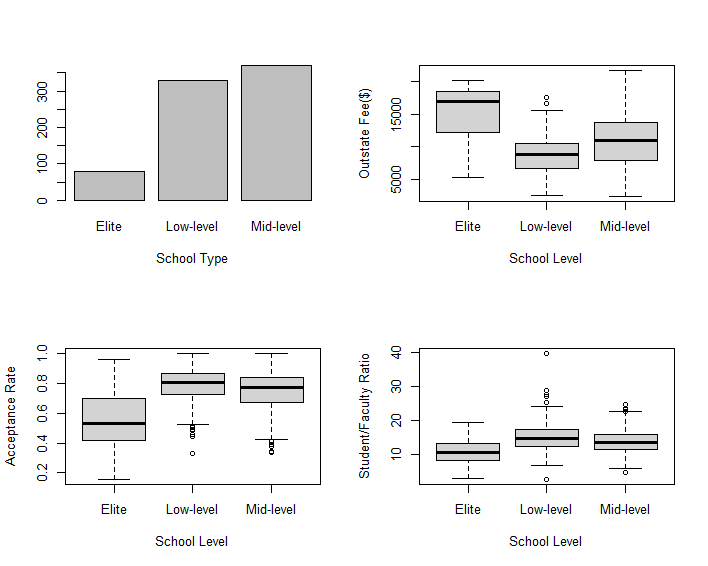
\includegraphics[width=1\linewidth]{Rplot.png}
    \caption{Enter Caption}
    \label{fig:enter-label}
\end{figure}

Starting from Figure 1, we observe that the number of Elite schools is almost half of the other school types as expected.
The second figure demonstrates that the Elite-level school fees for Outstate students are almost double those of other school types, and the third figure shows it is much harder to get into an Elite school. Hence, we can say that the acceptance rate and out-state fee are negatively correlated. The last figure is one way to explain the difference between Elite schools and other school types, which has the smallest Student/Faculty ratio which increases the student, academic relation.

\subsubsection{}
\textbf{Quantitative predictors}: "mpg", "cylinders", "displacement", "horsepower", "weight", "acceleration", "year", "origin" \\
\textbf{Qualitative predictors}: "name"\\
\textbf{Ranges}:
mpg:[9 46.6]\\
cylinders: [3,8]\\
displacement: [68,455]\\
horsepower: [46,230]\\
weight: [1613, 5140]\\
acceleration: [8,24.8]\\
year: [70,82]\\
origin: [1,3]
\begin{table}[htbp]
  \centering
  \caption{Mean and Std} 
  \label{tab:example}
  \begin{tabular}{|c|c|c|c|c|}
    \hline
    \textbf{Variable} & \textbf{Mean} & \textbf{Std.} &
    \textbf{New Mean}&
    \textbf{New Std.}\\
    \hline
    mpg & 23.45 & 7.83 & 24.40 & 7.83 \\
    \hline
    cylinders & 5.472 & 1.70 & 5.373 &  1.70\\
    \hline
    displacement & 194.4 & 104.38 & 187.2 & 104 \\
    \hline
    horsepower & 104.5 & 38.49 & 100.7 & 35.71\\
    \hline
    weight & 2978 & 847.9 & 2936 & 847.9 \\
    \hline
    acceleration & 15.54 & 2.75 & 15.73 & 2.75\\
    \hline
    year & 75.99 & 3.69 & 77.15 & 3.69\\
    \hline
    origin & 1.577 & 0.8 & 1.60 & 0.80\\
    \hline
  \end{tabular}
\end{table} \\

\begin{figure}[h]
    \centering
    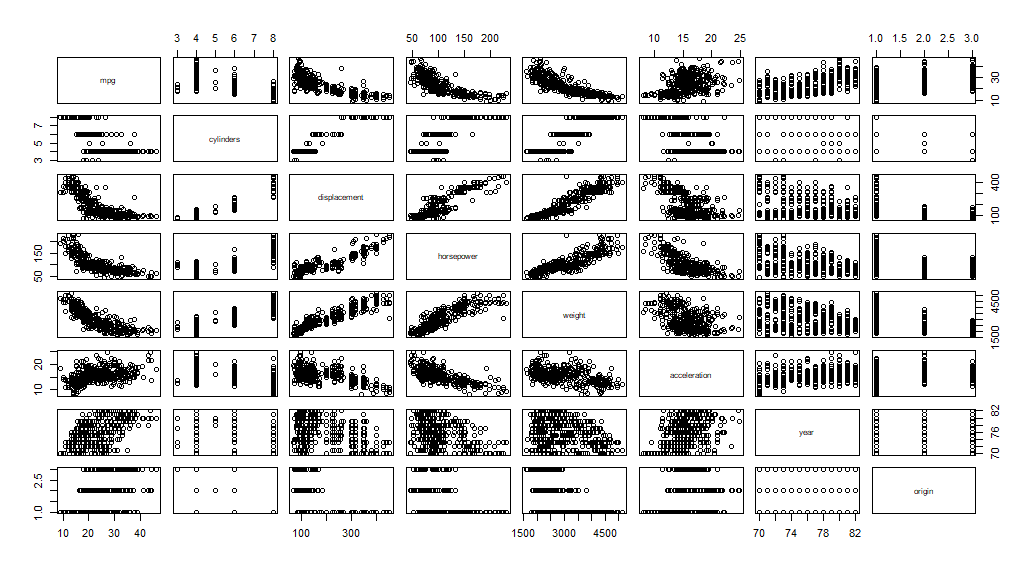
\includegraphics[width=1.25\linewidth]{Auto Pairs.png}
    \caption{Pair Plots of Auto}
    \label{fig:enter-label}
\end{figure}
By looking at the pair plots, we observe many correlations between variables. Such as mpg~displacement, horsepower~acceleration, etc. \\ \\

\begin{figure}
    \centering
    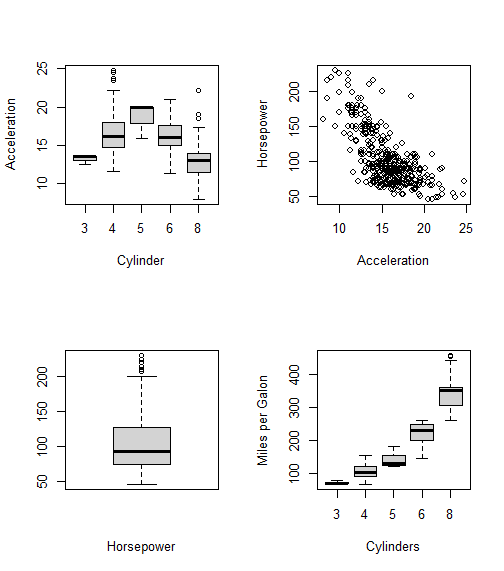
\includegraphics[width=1.25\linewidth]{Auto Plots.png}
    \caption{Plots}
    \label{fig:enter-label}
\end{figure}

Examining some of the plots that I have created, we can easily observe the correlations. In the first figure, the number of cylinders is used as a categorical variable and we see a polynomial behavior rather than a linear one. In the second plot, there exists a strong negative correlation between Horsepower and Acceleration as expected. More horsepower means less time to go from 0-100. Also, the variance of error terms seems close enough to deter heteroscedasticity problems. The third plot is straightforward, there are some outliers but most of the cars lie between 80-130 horsepower. Lastly, as the number of cylinders increases, the miles per gallon stat also increases. So another positive correlation is captured.

Just by looking at the pair plots, we can see that many variables can be used to predict mpg. Displacement has a negative correlation with mpg as well as horsepower and weight. Also, not so strongly but acceleration has a positive correlation with mpg. Lastly, the year shows the best correlation with mpg.
\end{document}
